\documentclass[14pt, a4paper]{report}
\usepackage{mathtext}
\usepackage[T2A]{fontenc}
\usepackage[utf8]{inputenc}
\usepackage[russian]{babel}
\usepackage{multirow}
\usepackage{slashbox}
\usepackage{makecell}
\usepackage{graphicx}
\usepackage{physics}
\usepackage{amstext}
\usepackage{caption}
\usepackage{subcaption}

\renewcommand{\thesection}{\arabic{section}.}
\renewcommand{\thesubsection}{\arabic{section}.\arabic{subsection}.}

\title{\textbf{Отчет о выполнении лабораторной работы 3.4.5 "Петля гистерезиса (динамический метод)"}}
\author{Алпатова Александра и Калашников Михаил, Б03-205}
\date{}

\begin{document}
\maketitle

\textbf{Цель работы:}
изучение петель гистерезиса различных ферромагнитных материалов в переменных полях.
\newline

\textbf{В работе используются:}
\begin{itemize}
\item автотрансформатор;
\item понижающий трансформатор;
\item интегрирующая цепочка;
\item амперметр;
\item вольтметр;
\item электронный осциллограф;
\item делитель напряжения;
\item тороидальные образцы с двумя обмотками;
\end{itemize}

\section{Теоретические сведения}



\section{Экспериментальная установка}



\section{Проведение эксперимента и обработка данных}

\begin{enumerate}

\setcounter{enumi}{0}

\item Соберем требуемую схему и подготовим к работе измерительные приборы.

\item С помощью потенциометра подберем такой ток питания, чтобы на экране ЭО наблюдалась предельная петля гистерезиса.

\item Подберем коэффициенты усиления ЭО так, чтобы петля занимала большую часть экрана.

\begin{table}[h!]
\centering
\begin{tabular}{| c | c | c |}
\hline
n & $K_X,\ мВ/дел$ & $K_Y,\ мВ/дел$ \\
\hline
1 & 20 & 50 \\
2 & 5 & 5 \\
3 & 100 & 20 \\
\hline
\end{tabular}
\caption{К пункту 3}
\end{table}

\item Проведем измерения полной шириины $2X_s$ и высоты $2Y_s$ предельной петли для каждой из катушек.

\item Также проведем измерения двойных амплитуд коэрцитивного $2X_c$ поля и остаточной индукции $2Y_r$.

\begin{table}[!h]
\centering
\begin{tabular}{| c | c | c | c | c |}
\hline
n & $2X_s,\ дел$ & $2Y_s,\ дел$ & $2X_c,\ дел$ & $2Y_r,\ дел$ \\
\hline
1 & $5.4\pm0.2$ & $2.6\pm0.2$ & $4.6\pm0.2$ & $2.6\pm0.2$ \\
2 & $4.4\pm0.2$ & $7.8\pm0.2$ & $2.6\pm0.2$ & $4.8\pm0.2$ \\
3 & $5.2\pm0.2$ & $6.4\pm0.2$ & $1.2\pm0.2$ & $3.0\pm0.2$ \\
\hline
\end{tabular}
\caption{К пункту 5}
\end{table}

\item Снимем положения вершин частных петель, плавно уменьшая ток намагничивания.

\item Расчитаем цену деления ЭО для каждого из образцов.	

\begin{table}[h!]
\centering
\begin{tabular}{| c | c | c |}
\hline
n & $H,\ \frac{А/м}{дел}$ & $B,\ \frac{Тл}{дел}$ \\
\hline
1 & 2.13 & 1.01 \\
2 & 0.90 & 0.02 \\
3 & 18.2 & 0.20 \\
\hline
\end{tabular}
\caption{К пункту 7}
\end{table}

\item Повторим все измерения для остальных катушек.

\item Проведем калибровку горизонтальной оси ЭО. "Закоротим" обмотку, подберем ток через сопротивление $R_0$ и рассчитаем чувствительность канала X по формуле $K_x=2R_0\sqrt{2}I_{эф}/(2x)$.

\begin{table}[h!]
\centering
\begin{tabular}{| c | c | c | c |}
\hline
n & $I_{ЭФ},\ А$ & $2x,\ дел$ & $K_x,\ мВ/дел$ \\
\hline
1 & $0.293\pm0.001$ & $8.8\pm0.2$ & $20.7\pm0.5$ \\
2 & $0.0812\pm0.0001$ & $9.6\pm0.2$ & $5.26\pm0.11$ \\
3 & $1.398\pm0.001$ & $7.0\pm0.2$ & $124\pm4$ \\
\hline
\end{tabular}
\caption{К пункту 9}
\end{table}

\item Разберем цепь тороида и проведем калибровку оси Y с помощью мультиметра используя формулу $K_y=2\sqrt{2}U_{ЭФ}/(2y)$

\begin{table}[h!]
\centering
\begin{tabular}{| c | c | c | c |}
\hline
n & $U_{ЭФ},\ мВ$ & $2y,\ дел$ & $K_y,\ мВ/дел$ \\
\hline
1 & $66.8\pm0.1$ & $6.0\pm0.2$ & $31.5\pm1.1$ \\
2 & $14.0\pm0.1$ & $5.0\pm0.2$ & $7.9\pm0.3$ \\
3 & $79.6\pm0.1$ & $7.8\pm0.2$ & $28.9\pm0.7$ \\
\hline
\end{tabular}
\caption{К пункту 10}
\end{table}

Полученные в предыдущих двух пунктах коэффициенты несколько отличается от коэффициентов, выставленных на ЭО. В дальнейшей работе следовало бы использовать их.

\item Подключим ЭО ко входу интегрирующей ячейки. Определим входное напряжение: $U_{ВХ}=2y\cdot K_Y=7.2\pm0.2\ В.$

\item Соединим ЭО с выходом ячейки и аналогичным образом определим напряжение $U_{ВЫХ}=2y\cdot K_y=0.058\pm0.002\ В.$

\item Рассчитаем постоянную времени $\tau=RC=\frac{1}{2\pi\nu}\frac{U_{ВХ}}{U_{ВЫХ}}=0.395\pm0.017\ с$. Используя параметры $R_И$ и $C_И$ определим действительное значение постоянной времени $\tau_0=R_ИC_И=0.4\ c$. Проверим условие $R\gg\frac{1}{\omega C}\Leftrightarrow\omega RC\gg1$. Оно выполняется, так как $\omega R_ИC_И\approx130$.

\item Рассчитаем амплитуды для каждой из катушек.

\item Используя результаты измерений в пункте 4 рассчитаем амплитуду $H_{max}$, соответствующую состоянию насыщения и индукцию насещения $B_s$.

\item По результатам пункта 5 рассчитаем коэрцитивное поле $H_c$ и остаточную индукцию $B_r$.

\item По графику определим значения $\mu_{нач}$ и $\mu_{max}$.

\item Сведем результаты вычислений в таблицу.

\begin{table}[h!]
\centering
\begin{tabular}{| c | c | c | c |}
\hline
Ампл. & Fe-Ni & Феррит & Fe-Si \\
\hline
$H_c,\ \frac{А}{м}	$ & $4.9\pm0.4$ & $1.17\pm0.18$ & $11\pm4$ \\
$H_{c0},\ \frac{А}{м}$ & 5.6 & 4-100 & 40 \\
\hline
$B_s,\ Тл$ & $1.3\pm0.2$ & $0.065\pm0.003$ & $0.64\pm0.04$ \\
$B_{s0},\ Тл$ & 1.60 & 0.3-0.4 & 1.95 \\
\hline
$\mu_{нач}$ & $5.6\cdot10^4$ & $1.4\cdot10^4$ & $7.6\cdot10^3$ \\
$\mu_{нач0}$ & $1.2\cdot10^3$ & $500-2\cdot10^4$ & 500 \\
\hline
$\mu_{max}$ & $3.6\cdot10^7$ & $3.0\cdot10^4$ & $2.4\cdot10^4$ \\
$\mu_{max0}$ & $3.5\cdot10^3$ & $-$ & $7\cdot10^3$ \\
\hline
$H_{max},\ \frac{А}{м}$ & $5.7\pm0.4$ & $1.9\pm0.18$ & $47\pm4$ \\
\hline
$B_r,\ Тл$ & $1.3\pm0.2$ & $0.04\pm0.003$ & $0.3\pm0.04$ \\
\hline

\end{tabular}
\caption{К пункту 18}
\end{table}

\end{enumerate}

\section{Приложения}

\begin{figure}
	\centering
	\begin{subfigure}{.5\textwidth}
		\centering
		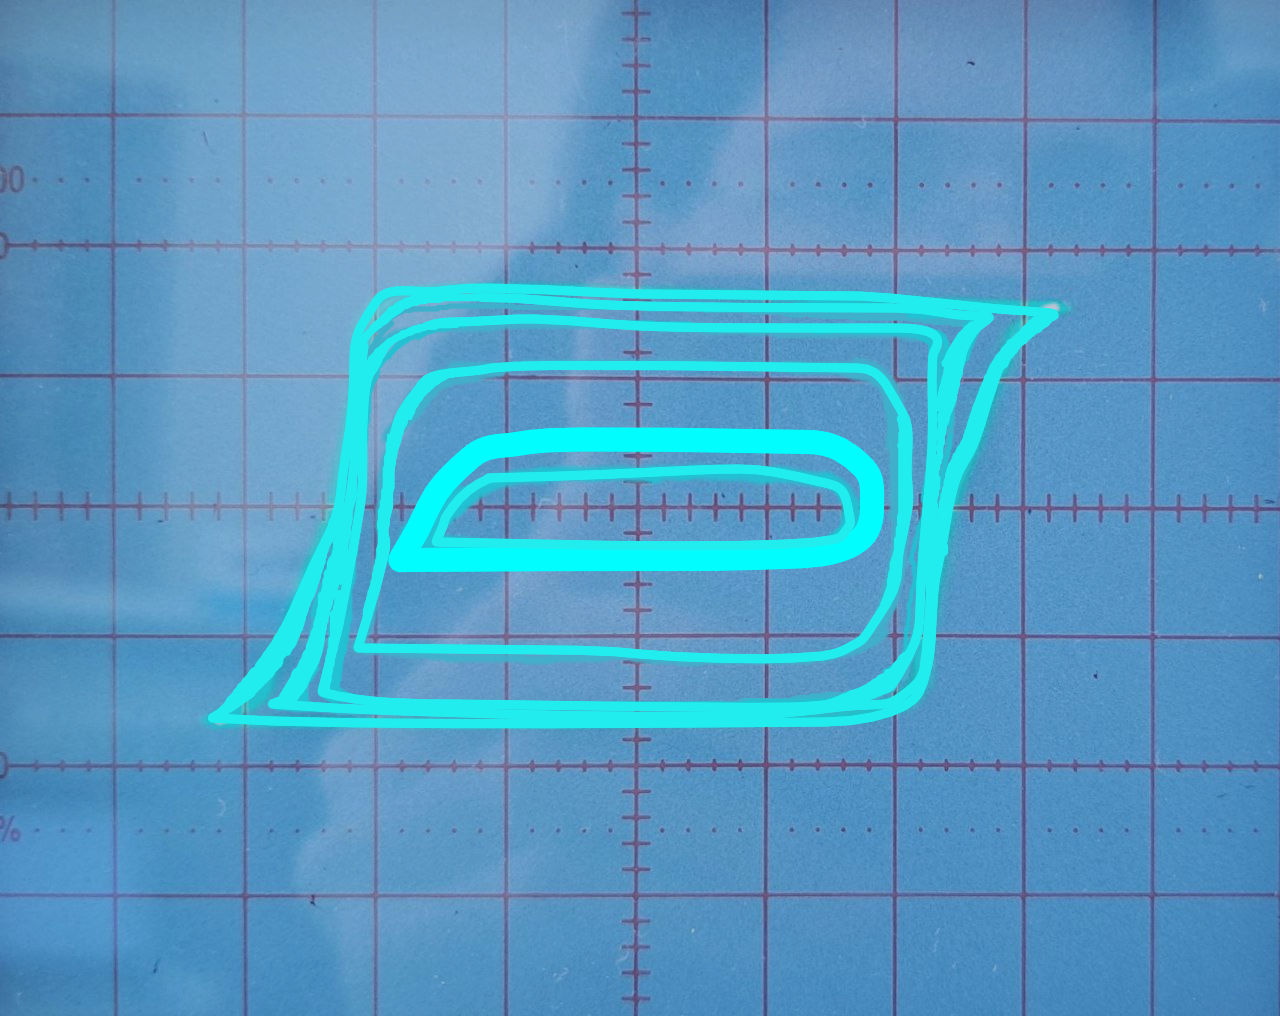
\includegraphics[width=\linewidth]{images/345_4.png}
	\end{subfigure}%
	\begin{subfigure}{.5\textwidth}
		\centering
		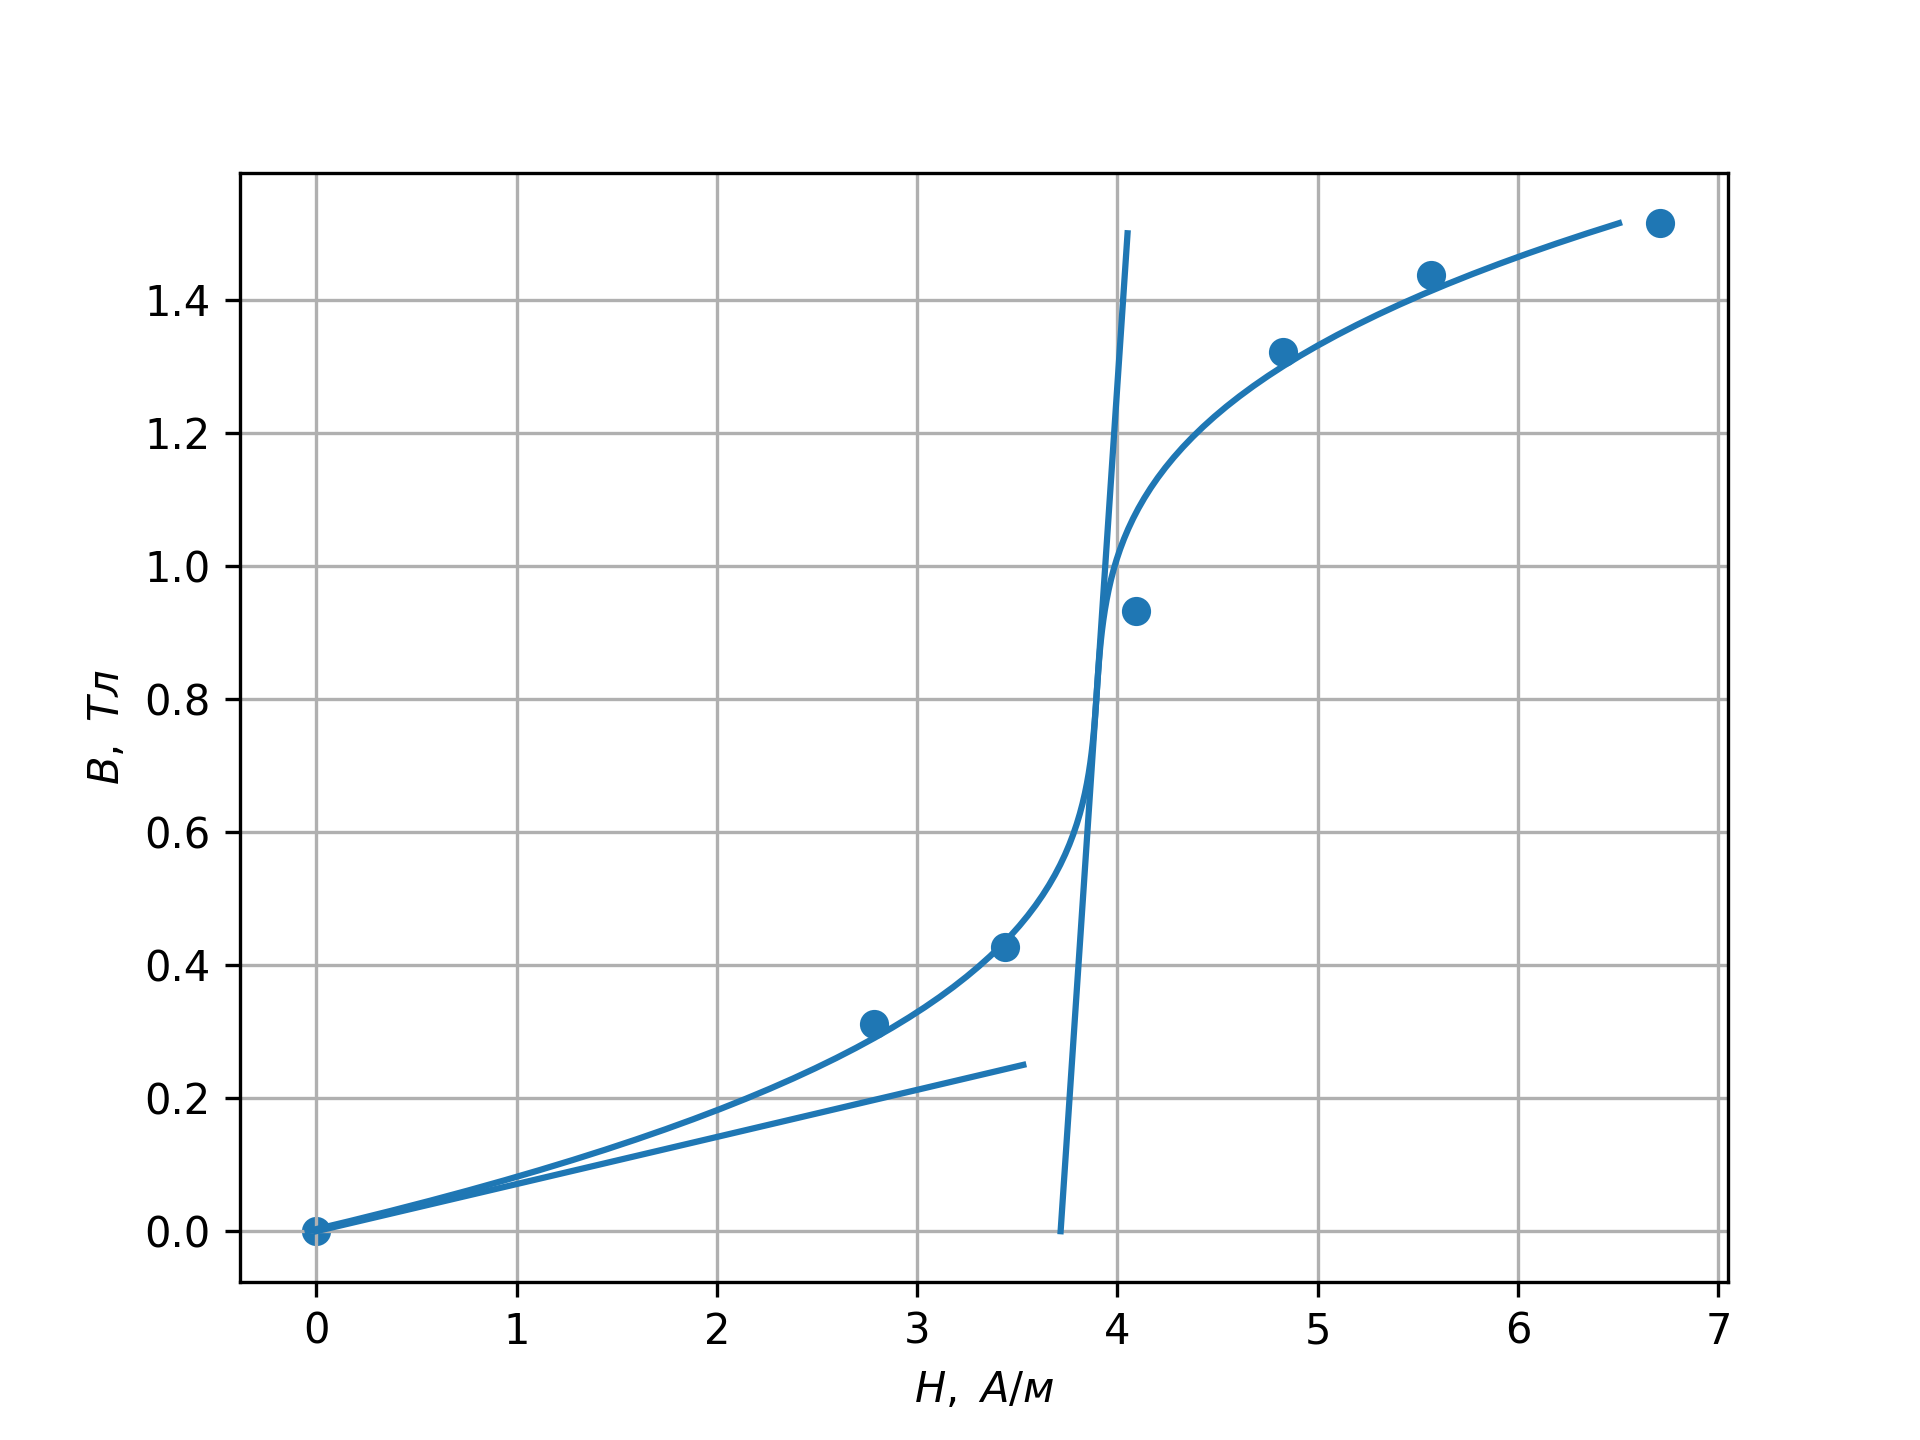
\includegraphics[width=\linewidth]{images/345_1.png}
	\end{subfigure}
	\caption{кривая гистерезиса и начальная кривая катушки из Fe-Ni}
\end{figure}

\begin{figure}
	\centering
	\begin{subfigure}{.5\textwidth}
		\centering
		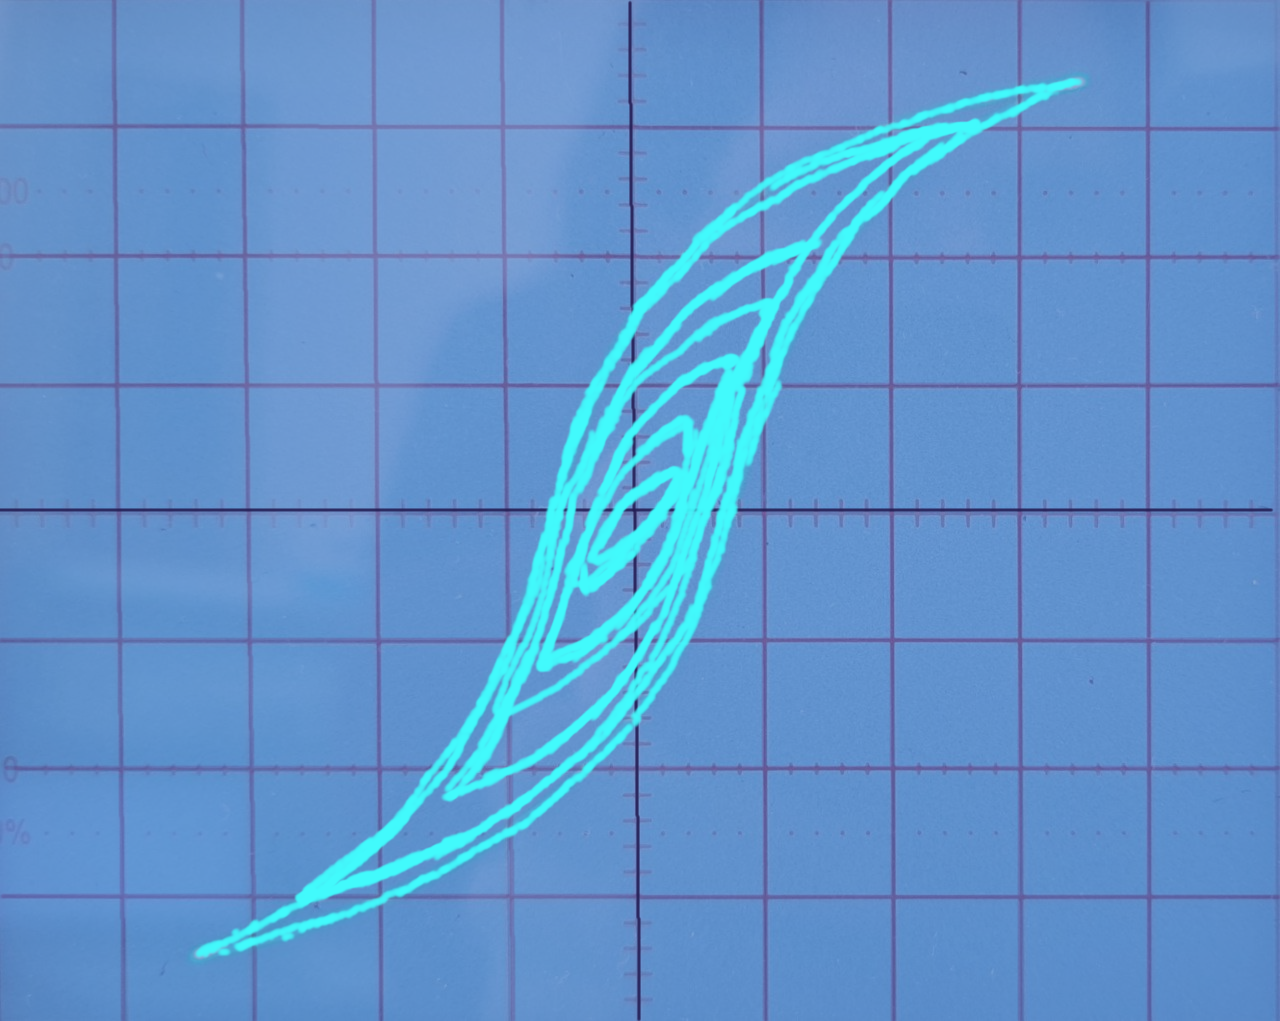
\includegraphics[width=\linewidth]{images/345_5.png}
	\end{subfigure}%
	\begin{subfigure}{.5\textwidth}
		\centering
		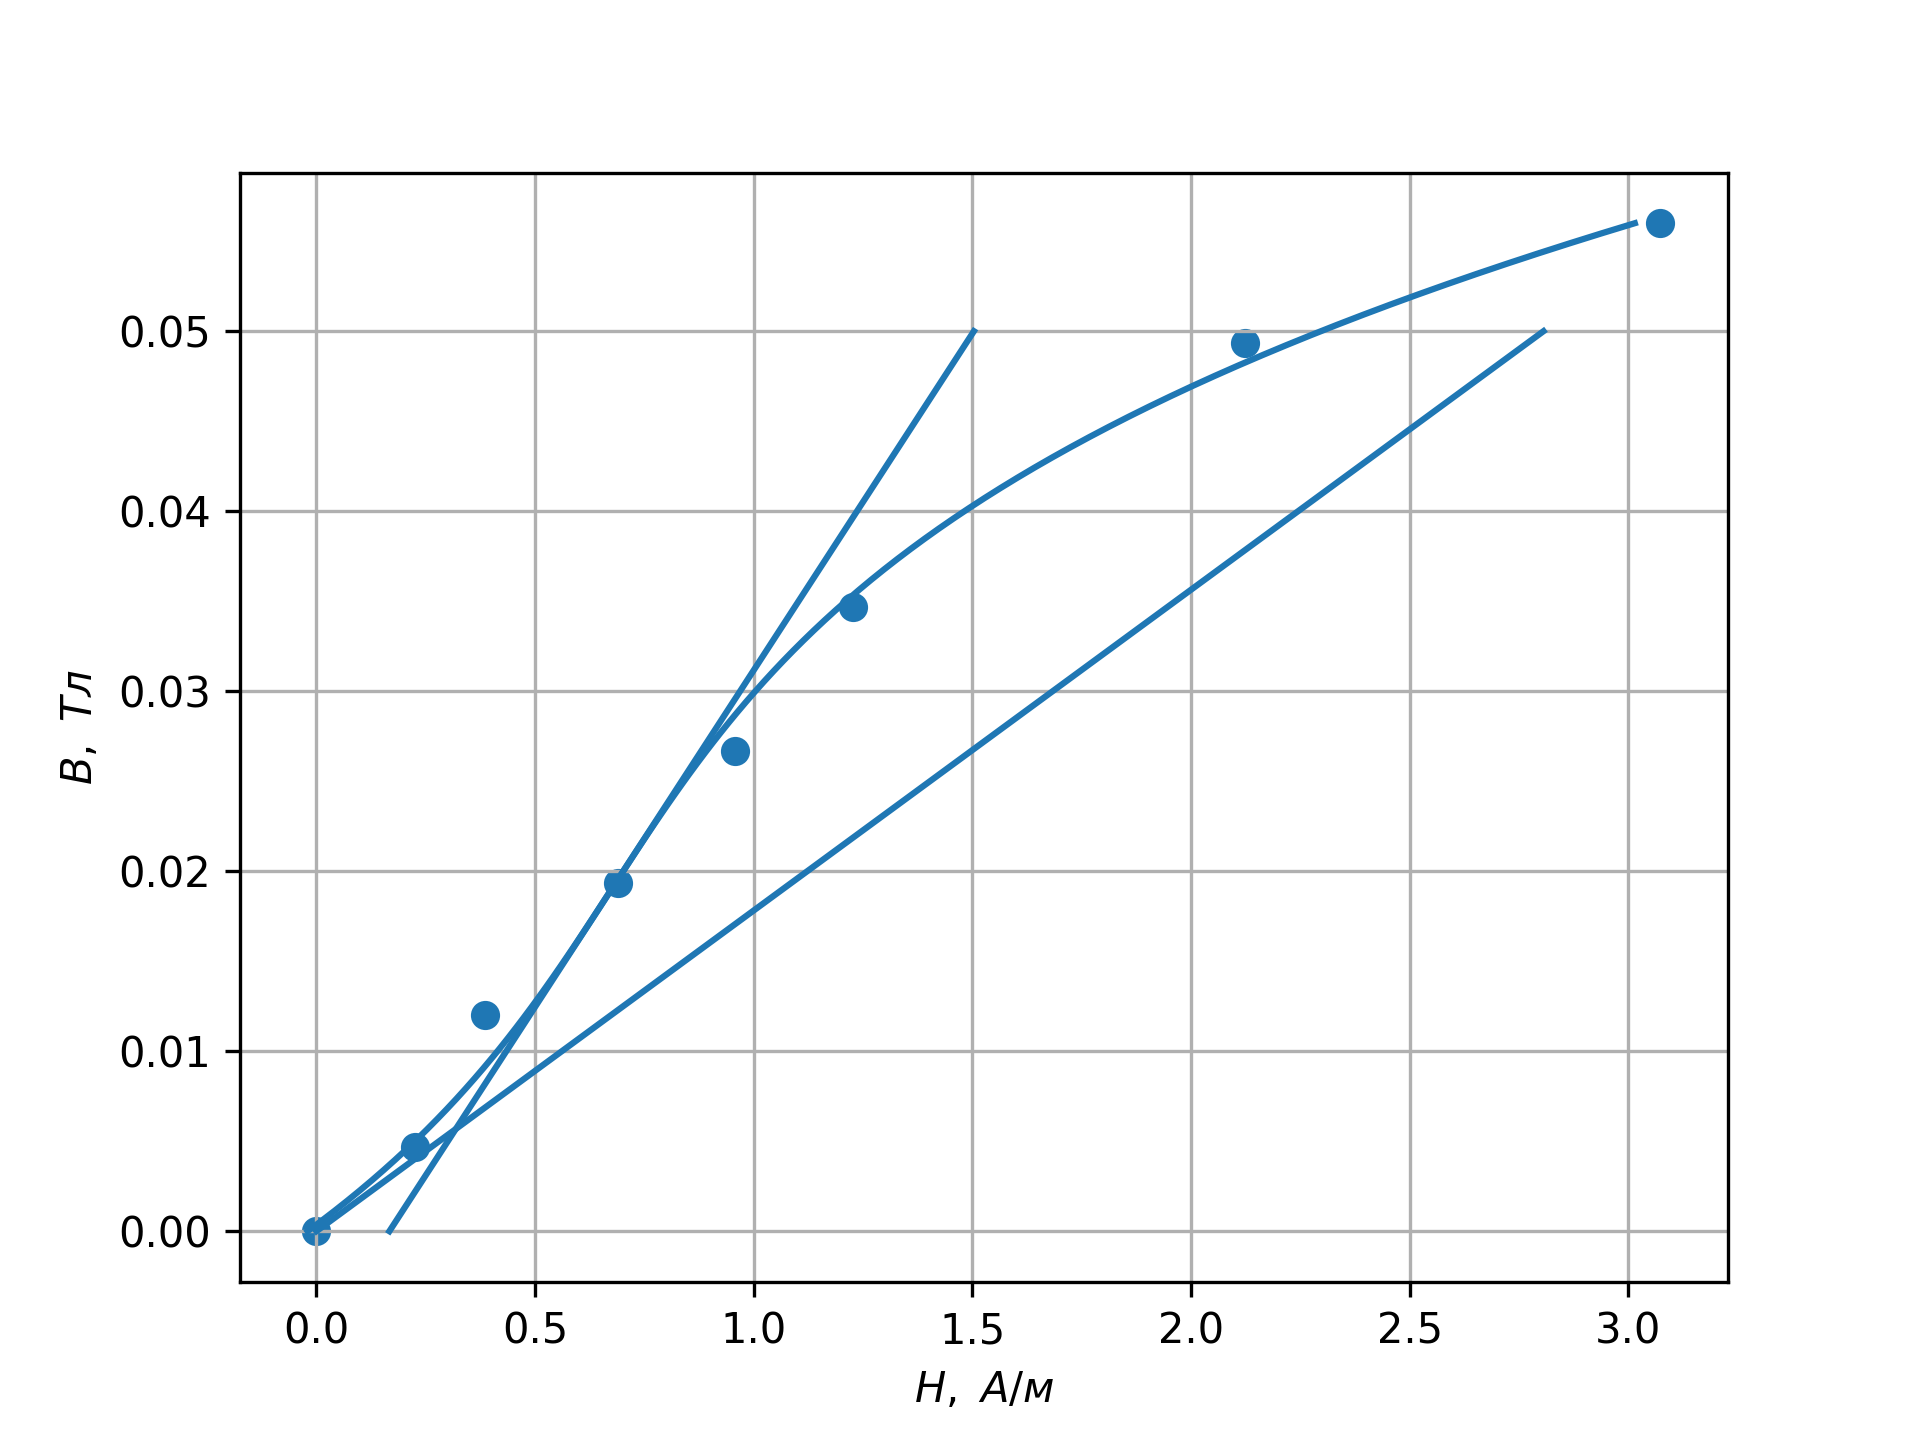
\includegraphics[width=\linewidth]{images/345_2.png}
	\end{subfigure}
	\caption{кривая гистерезиса и начальная кривая катушки из феррита}
\end{figure}

\begin{figure}
	\centering
	\begin{subfigure}{.5\textwidth}
		\centering
		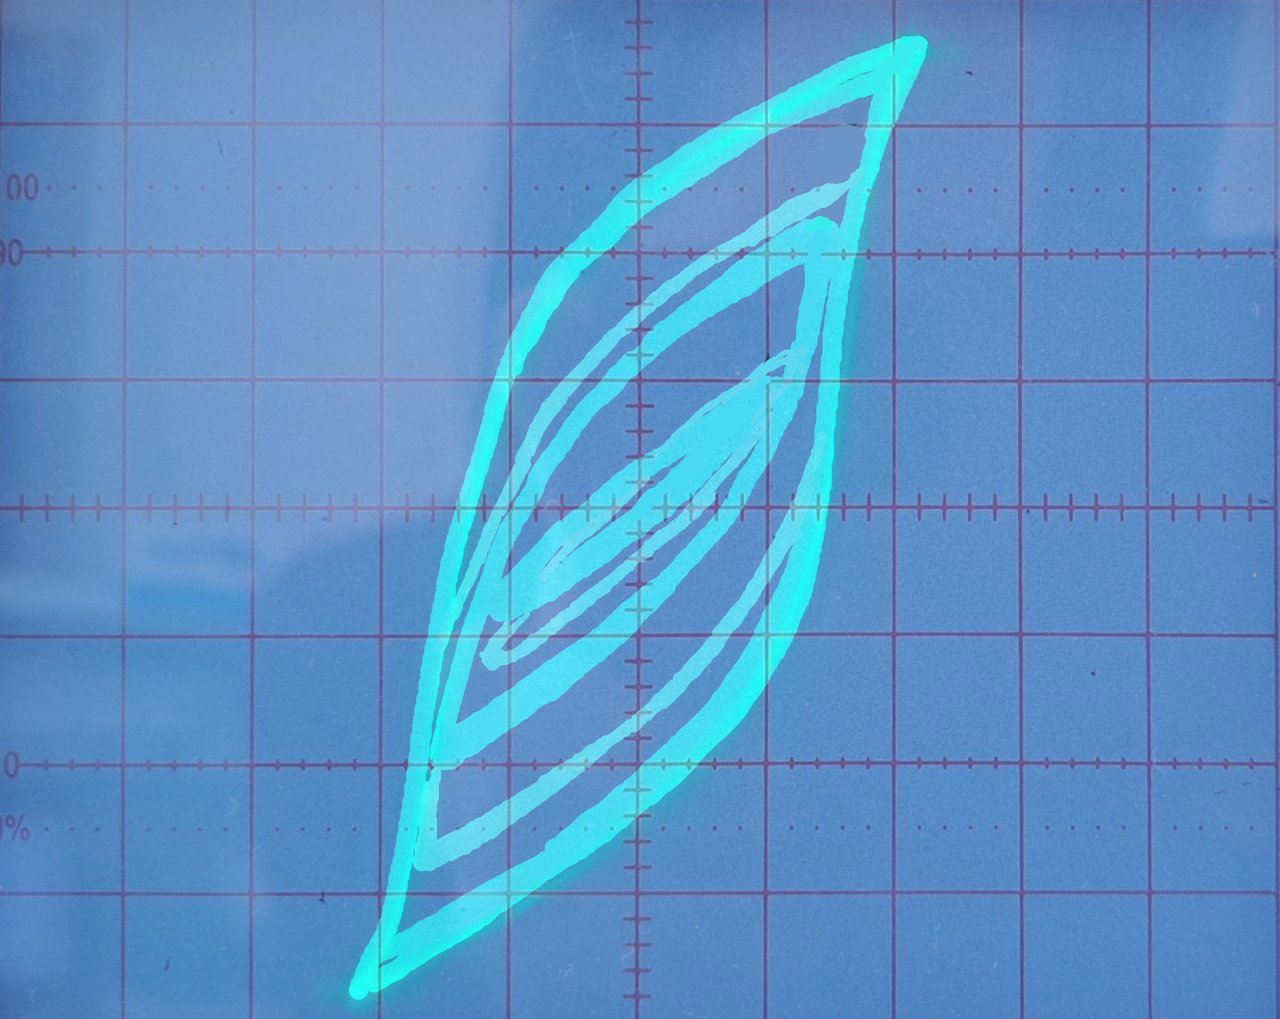
\includegraphics[width=\linewidth]{images/345_6.png}
	\end{subfigure}%
	\begin{subfigure}{.5\textwidth}
		\centering
		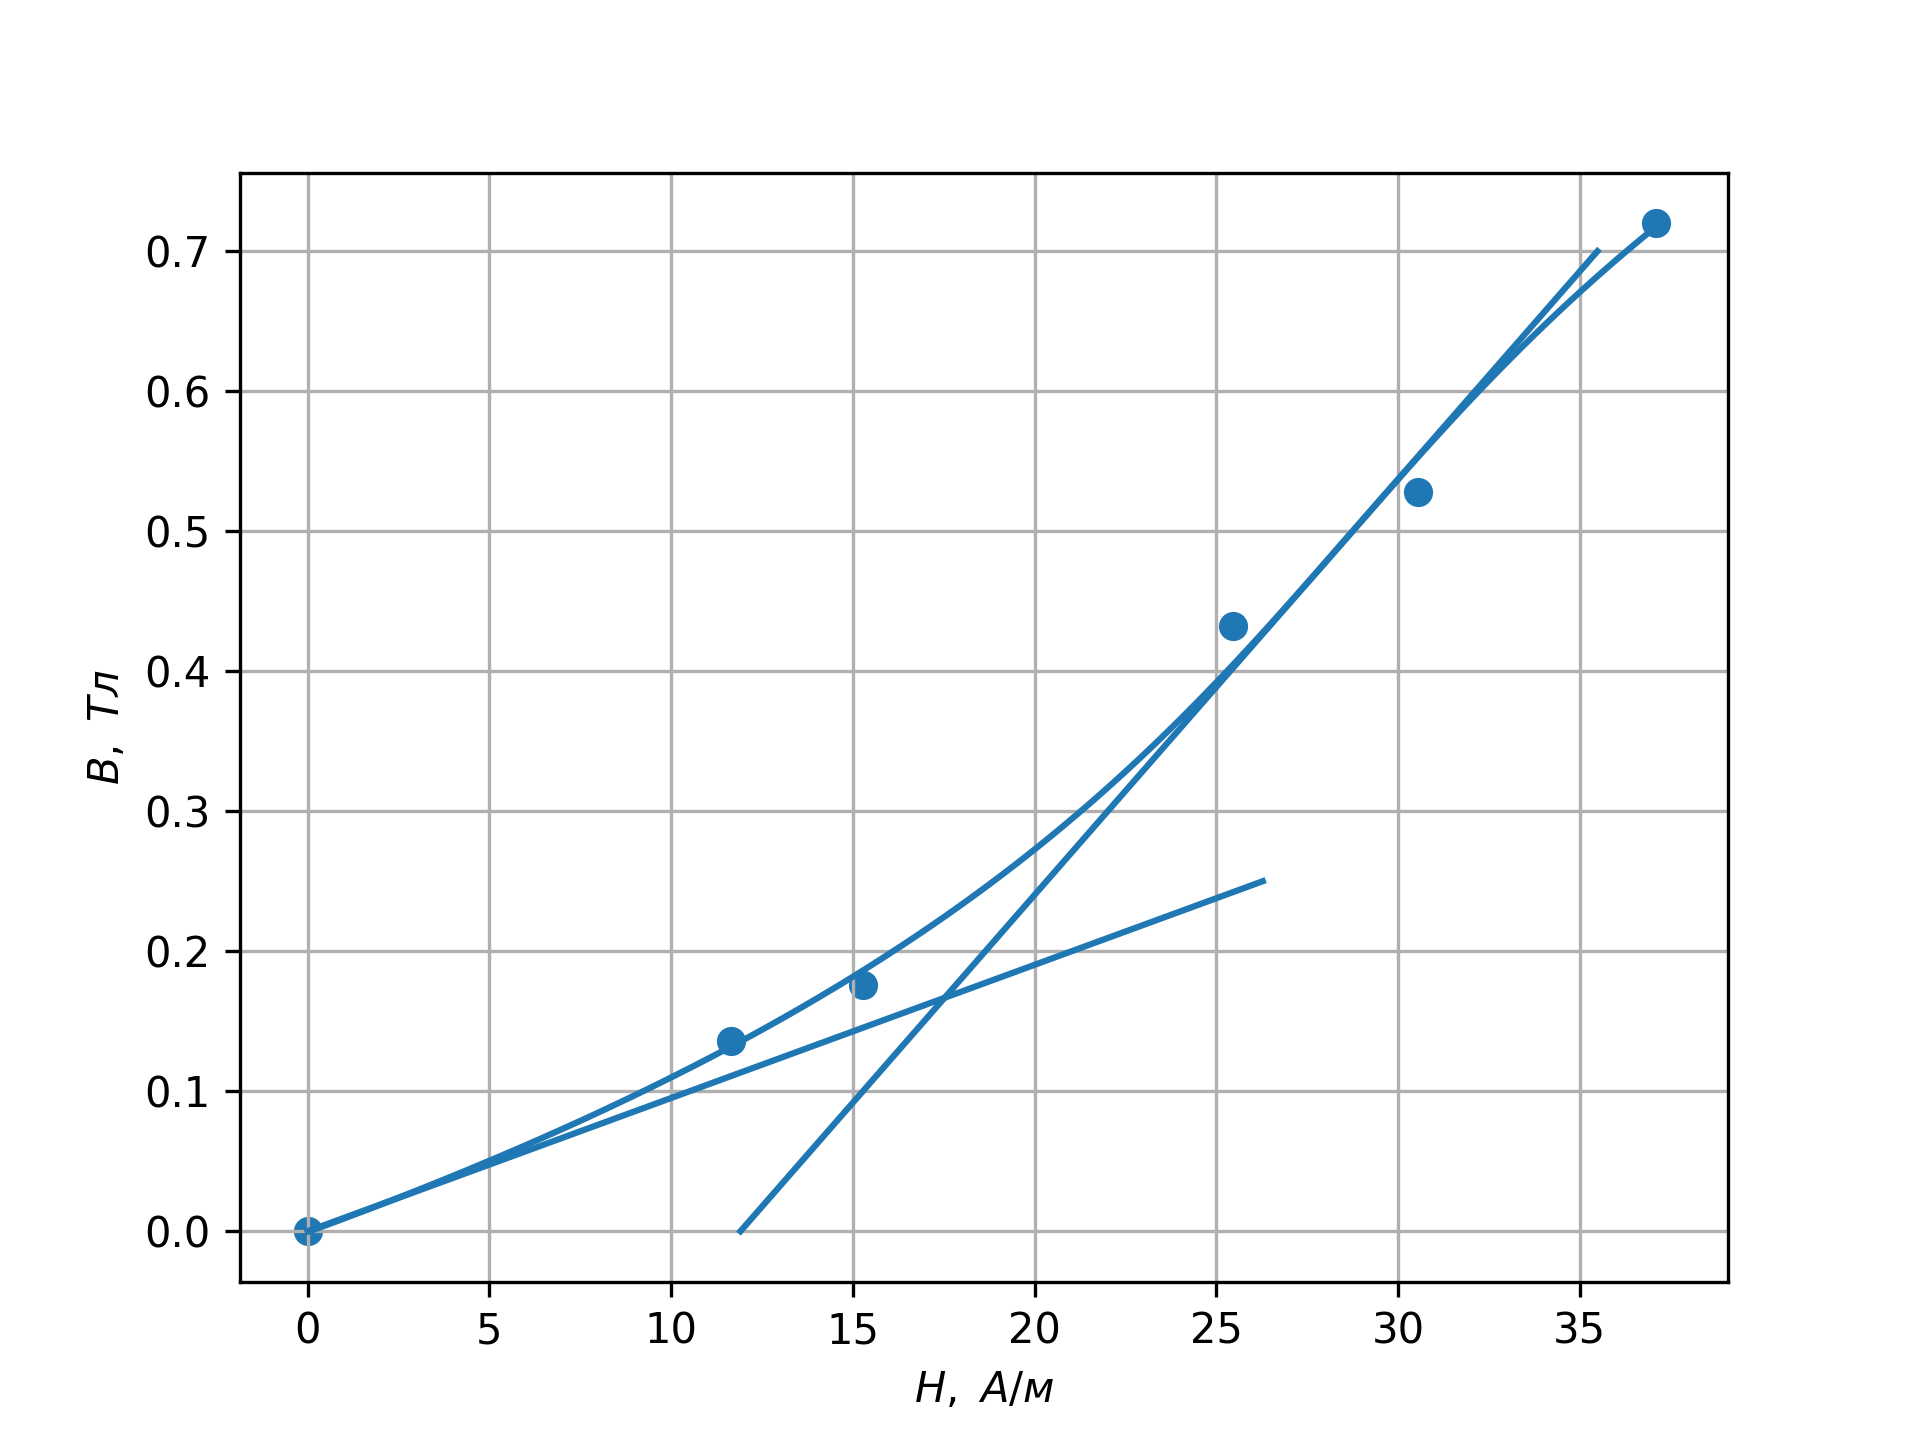
\includegraphics[width=\linewidth]{images/345_3.png}
	\end{subfigure}
	\caption{кривая гистерезиса и начальная кривая катушки из Fe-Si}
\end{figure}

\end{document}